\documentclass[german,ignorenonframetext]{beamer}

\usepackage[ngerman]{babel} % f�r deutsche Spracheinstellungen
\usepackage{graphics} % um Bilder einbinden zu k�nnen
\usepackage[dvips]{epsfig} % um Bilder zu skalieren
\usepackage[latin1]{inputenc} % inputencoding (MacOS) f�r Umlaute und Akzente

%%%%%%%%%%%%%%%%%%%%%%%%%%%%%%%%%%%%%%%%%%%

%%%%%%% Die folgenden Befehle definieren das Grundlayout, blenden auf der
%%%%%%% Titelseite die HAW-Infos ein und setzen das 
%%%%%%% HAW-Logo in die Ecke
\mode<presentation>{\usetheme{Berkeley}}
\logo{\pgfimage[height=1.5cm]{HAW_wuerfel+}}
\institute[MT -- HAW Hamburg]{HAW Hamburg\\ Dept. Informatik}

%%%%%%% der folgende Befehl l�sst die mit "\pause" verdeckten Teile der Folien 
%%%%%%% transparent erscheinen.  
\setbeamercovered{transparent}  

%%%%%%% die folgende Sequenz blendet mit jeder neuen Section einmal das 
%%%%%%% Inhaltsverzeichnis mit dem Titel "�bersicht" ein und markiert den
%%%%%%% jeweils aktuellen Gliederungspunkt
\AtBeginSection[]{
\begin{frame}<beamer>
\frametitle{�bersicht} 
\tableofcontents[currentsection,currentsubsection]
\end{frame}
}

%%%%%%%%%%%%%%%%%%%%%%%%%%%%%%%%%%%%%%%%%%%

%%%%%%% jeder dieser Titelseiten-Befehle kennt eine in eckige Klammern gesetzte 
%%%%%%% Kurzform, die im Rand benutzt wird
\title[�berschrift]{Anwendungen}
\subtitle{Gesten und Gedanken Steuerung}
\author[Koumenji Mohamed]{Mohamed Kemel Koumenji}
\date{\today}

%%%%%%%%%%%%%%%%%%%%%%%%%%%%%%%%%%%%%%%%%%%

\begin{document}

%%%%%% dieser Befehl erzeugt das Deckblatt. 
%%%%%% Mit der Option plain wird das Layout f�r das Deckblatt abgeschaltet
%\frame[plain]{\titlepage}
\frame{\titlepage}

\begin{frame}
  \frametitle{�bersicht}
  \tableofcontents
\end{frame}

%%%%%%%%%%%%%%%%%%%%%%%%%%%%%%%%%%%%%%%%%%%
\section{Hardware} % die sections sind hier nur zum Strukturieren des Vortrags!!
%% der Name der section taucht nur im Inhaltsverzeichnis und im linken Rand auf.
%%%%%%%%%%%%%%%%%%%%%%%%%%%%%%%%%%%%%%%%%%%
\begin{frame}
\frametitle{Brain Control Interface (BCI)}

Das BCI ist ein 1-Kanal EEG-Headset.
Erfasst Entspannung- und Aufmerksamkeit auf Basis von EEG-Messungen.
 

\begin{figure}
	\centering
		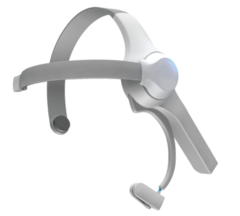
\includegraphics[scale=0.50]{MindWave.png}
	\caption{Neurosky-Mindwave}
	\label{fig:MindWave}
\end{figure}




\end{frame}


\begin{frame}
\frametitle{Microsoft Kinect}
Die Kinect ist ein Sensor f�r Bilderfassung.\\
Der Tiefensensor, hat einen IR-Laserprojektor sowie ein CMOS Monochrom-Kameramodul.







\begin{figure}
	\centering
		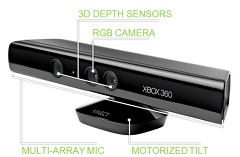
\includegraphics[scale=0.70]{KinectSensor}
	\caption{Microsoft-Kinect}
	\label{fig:KinectSensor}
\end{figure}


\end{frame}


%%%%%%%%%%%%%%%%%%%%%%%%%%%%%%%%%%%%%%%%%%%
\section{Abstrakte Kunst}
%%%%%%%%%%%%%%%%%%%%%%%%%%%%%%%%%%%%%%%%%%%
\begin{frame}

\frametitle{Mit den H�nden malen und mit den Gedanken f�rben}       

%\begin{columns}
%\column{.4\textwidth}
%\begin{center}
%\pgfimage[height = 1\textwidth]{code} \\
%\scriptsize
%	Abstrakte Kunst
%\end{center}
%\end{columns}

\begin{figure}
	\centering
		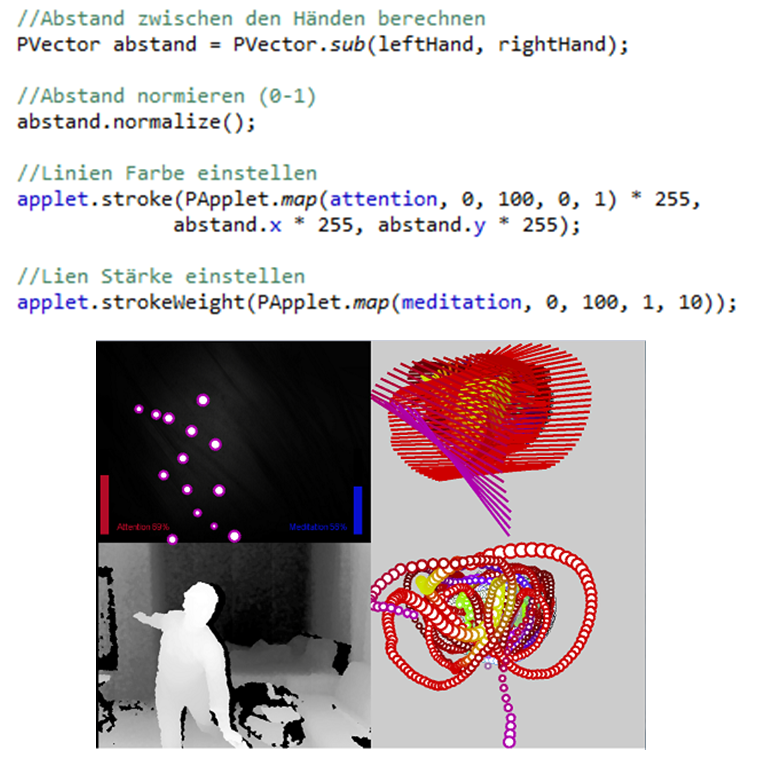
\includegraphics[width=0.60\textwidth]{code.PNG}
	\caption{Abstrakte Kunst}
	\label{fig:code}
\end{figure}



\end{frame}


%%%%%%%%%%%%%%%%%%%%%%%%%%%%%%%%%%%%%%%%%%%
\section{Audio Aufnahme und Steuerung von Gitarreneffekte}
%%%%%%%%%%%%%%%%%%%%%%%%%%%%%%%%%%%%%%%%%%%

\begin{frame}

\frametitle{Playing Music}


\begin{figure}
	\centering
		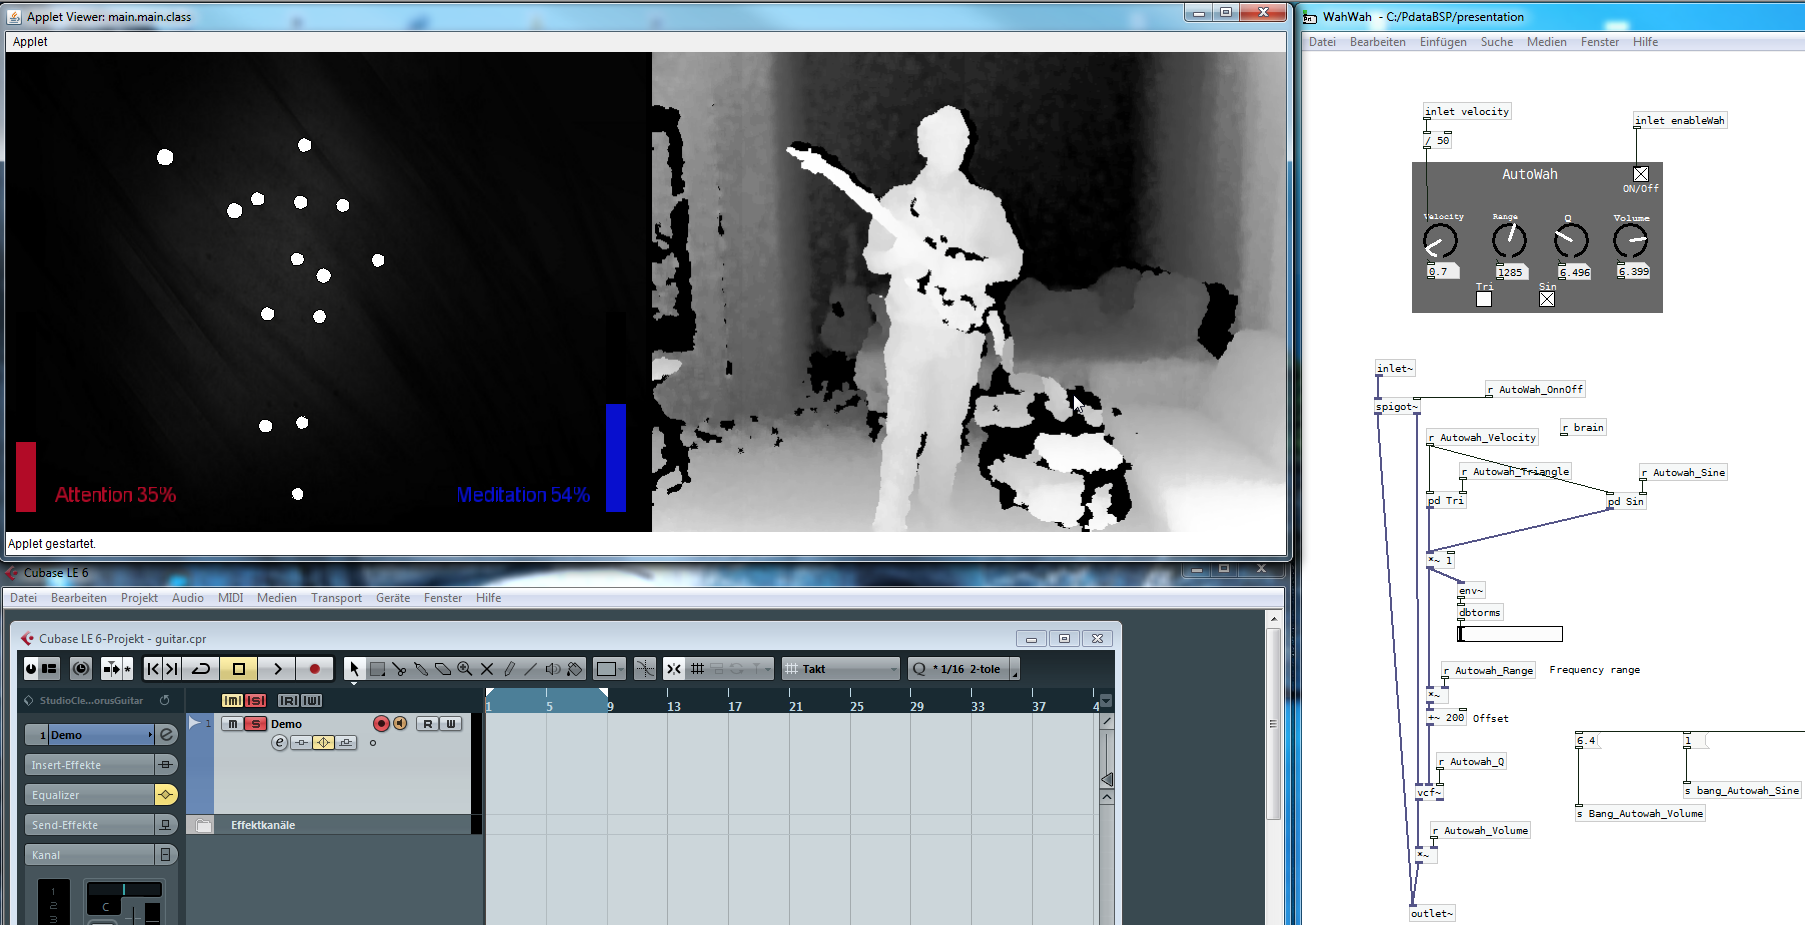
\includegraphics[scale=0.20]{Audio.PNG}
	\caption{schnappschuss aus dem Video [Carlos Santana-Europa(cover)]}
	\label{fig:Audio}
\end{figure}




\end{frame}

\end{document}




%%%%%%%%%%%%%%%%%%%%%%%%%%%%%%%%%%%%%%%%%%%
%%  besondere Gestaltungselemente f�r Vortragsfolien
%%%%%%%%%%%%%%%%%%%%%%%%%%%%%%%%%%%%%%%%%%%

% Folie
\begin{frame}
\frametitle{Folientitel}
        Text, Bilder, Bl�cke
\end{frame}

% neutraler Kasten
\begin{block}{Blocktitel}
        Blocktext
\end{block}

% gr�ner Kasten
\begin{exampleblock}{Beispielblocktitel}
        Beispielblocktext
\end{exampleblock}

% roter Kasten
\begin{alertblock}{Warnungsblocktitel}
        Warnungsblocktext
\end{alertblock}

% mehrspaltige Folie mit variablen Spaltenbreiten
\begin{columns}
\column{.55\textwidth}
        Text oder Bild
\column{.45\textwidth}
        Text oder Bild
\end{columns}

% sukzessiver Folienaufbau 
\pause

% mehr Befehle f�r sukzessiven Folienaufbau, 
% der geklammerte Teil erscheint jeweils ab der dritten Teil-Folie
\uncover<3->{}
\only<3->{}
\invisible<1-2>{}

% rote Markierung des geklammerten Teils bei der vierten Teil-Folie
\alert<4>{}

%%%%%%%%%%%%%%%%%%%%%%%%%%%%%%%%%%%%%%%%%%%